% Options for packages loaded elsewhere
\PassOptionsToPackage{unicode}{hyperref}
\PassOptionsToPackage{hyphens}{url}
%
\documentclass[
]{article}
\title{Lec05\_classnote\_LS}
\author{shuna}
\date{1/28/2022}

\usepackage{amsmath,amssymb}
\usepackage{lmodern}
\usepackage{iftex}
\ifPDFTeX
  \usepackage[T1]{fontenc}
  \usepackage[utf8]{inputenc}
  \usepackage{textcomp} % provide euro and other symbols
\else % if luatex or xetex
  \usepackage{unicode-math}
  \defaultfontfeatures{Scale=MatchLowercase}
  \defaultfontfeatures[\rmfamily]{Ligatures=TeX,Scale=1}
\fi
% Use upquote if available, for straight quotes in verbatim environments
\IfFileExists{upquote.sty}{\usepackage{upquote}}{}
\IfFileExists{microtype.sty}{% use microtype if available
  \usepackage[]{microtype}
  \UseMicrotypeSet[protrusion]{basicmath} % disable protrusion for tt fonts
}{}
\makeatletter
\@ifundefined{KOMAClassName}{% if non-KOMA class
  \IfFileExists{parskip.sty}{%
    \usepackage{parskip}
  }{% else
    \setlength{\parindent}{0pt}
    \setlength{\parskip}{6pt plus 2pt minus 1pt}}
}{% if KOMA class
  \KOMAoptions{parskip=half}}
\makeatother
\usepackage{xcolor}
\IfFileExists{xurl.sty}{\usepackage{xurl}}{} % add URL line breaks if available
\IfFileExists{bookmark.sty}{\usepackage{bookmark}}{\usepackage{hyperref}}
\hypersetup{
  pdftitle={Lec05\_classnote\_LS},
  pdfauthor={shuna},
  hidelinks,
  pdfcreator={LaTeX via pandoc}}
\urlstyle{same} % disable monospaced font for URLs
\usepackage[margin=1in]{geometry}
\usepackage{color}
\usepackage{fancyvrb}
\newcommand{\VerbBar}{|}
\newcommand{\VERB}{\Verb[commandchars=\\\{\}]}
\DefineVerbatimEnvironment{Highlighting}{Verbatim}{commandchars=\\\{\}}
% Add ',fontsize=\small' for more characters per line
\usepackage{framed}
\definecolor{shadecolor}{RGB}{248,248,248}
\newenvironment{Shaded}{\begin{snugshade}}{\end{snugshade}}
\newcommand{\AlertTok}[1]{\textcolor[rgb]{0.94,0.16,0.16}{#1}}
\newcommand{\AnnotationTok}[1]{\textcolor[rgb]{0.56,0.35,0.01}{\textbf{\textit{#1}}}}
\newcommand{\AttributeTok}[1]{\textcolor[rgb]{0.77,0.63,0.00}{#1}}
\newcommand{\BaseNTok}[1]{\textcolor[rgb]{0.00,0.00,0.81}{#1}}
\newcommand{\BuiltInTok}[1]{#1}
\newcommand{\CharTok}[1]{\textcolor[rgb]{0.31,0.60,0.02}{#1}}
\newcommand{\CommentTok}[1]{\textcolor[rgb]{0.56,0.35,0.01}{\textit{#1}}}
\newcommand{\CommentVarTok}[1]{\textcolor[rgb]{0.56,0.35,0.01}{\textbf{\textit{#1}}}}
\newcommand{\ConstantTok}[1]{\textcolor[rgb]{0.00,0.00,0.00}{#1}}
\newcommand{\ControlFlowTok}[1]{\textcolor[rgb]{0.13,0.29,0.53}{\textbf{#1}}}
\newcommand{\DataTypeTok}[1]{\textcolor[rgb]{0.13,0.29,0.53}{#1}}
\newcommand{\DecValTok}[1]{\textcolor[rgb]{0.00,0.00,0.81}{#1}}
\newcommand{\DocumentationTok}[1]{\textcolor[rgb]{0.56,0.35,0.01}{\textbf{\textit{#1}}}}
\newcommand{\ErrorTok}[1]{\textcolor[rgb]{0.64,0.00,0.00}{\textbf{#1}}}
\newcommand{\ExtensionTok}[1]{#1}
\newcommand{\FloatTok}[1]{\textcolor[rgb]{0.00,0.00,0.81}{#1}}
\newcommand{\FunctionTok}[1]{\textcolor[rgb]{0.00,0.00,0.00}{#1}}
\newcommand{\ImportTok}[1]{#1}
\newcommand{\InformationTok}[1]{\textcolor[rgb]{0.56,0.35,0.01}{\textbf{\textit{#1}}}}
\newcommand{\KeywordTok}[1]{\textcolor[rgb]{0.13,0.29,0.53}{\textbf{#1}}}
\newcommand{\NormalTok}[1]{#1}
\newcommand{\OperatorTok}[1]{\textcolor[rgb]{0.81,0.36,0.00}{\textbf{#1}}}
\newcommand{\OtherTok}[1]{\textcolor[rgb]{0.56,0.35,0.01}{#1}}
\newcommand{\PreprocessorTok}[1]{\textcolor[rgb]{0.56,0.35,0.01}{\textit{#1}}}
\newcommand{\RegionMarkerTok}[1]{#1}
\newcommand{\SpecialCharTok}[1]{\textcolor[rgb]{0.00,0.00,0.00}{#1}}
\newcommand{\SpecialStringTok}[1]{\textcolor[rgb]{0.31,0.60,0.02}{#1}}
\newcommand{\StringTok}[1]{\textcolor[rgb]{0.31,0.60,0.02}{#1}}
\newcommand{\VariableTok}[1]{\textcolor[rgb]{0.00,0.00,0.00}{#1}}
\newcommand{\VerbatimStringTok}[1]{\textcolor[rgb]{0.31,0.60,0.02}{#1}}
\newcommand{\WarningTok}[1]{\textcolor[rgb]{0.56,0.35,0.01}{\textbf{\textit{#1}}}}
\usepackage{graphicx}
\makeatletter
\def\maxwidth{\ifdim\Gin@nat@width>\linewidth\linewidth\else\Gin@nat@width\fi}
\def\maxheight{\ifdim\Gin@nat@height>\textheight\textheight\else\Gin@nat@height\fi}
\makeatother
% Scale images if necessary, so that they will not overflow the page
% margins by default, and it is still possible to overwrite the defaults
% using explicit options in \includegraphics[width, height, ...]{}
\setkeys{Gin}{width=\maxwidth,height=\maxheight,keepaspectratio}
% Set default figure placement to htbp
\makeatletter
\def\fps@figure{htbp}
\makeatother
\setlength{\emergencystretch}{3em} % prevent overfull lines
\providecommand{\tightlist}{%
  \setlength{\itemsep}{0pt}\setlength{\parskip}{0pt}}
\setcounter{secnumdepth}{-\maxdimen} % remove section numbering
\ifLuaTeX
  \usepackage{selnolig}  % disable illegal ligatures
\fi

\begin{document}
\maketitle

\hypertarget{central-limit-theorem}{%
\paragraph{Central Limit Theorem}\label{central-limit-theorem}}

\hypertarget{uniform-distribution}{%
\subparagraph{Uniform Distribution}\label{uniform-distribution}}

\begin{Shaded}
\begin{Highlighting}[]
\FunctionTok{mean}\NormalTok{(}\FunctionTok{runif}\NormalTok{(}\DecValTok{100}\NormalTok{, }\DecValTok{0}\NormalTok{,}\DecValTok{1}\NormalTok{))}
\end{Highlighting}
\end{Shaded}

\begin{verbatim}
## [1] 0.5202566
\end{verbatim}

\begin{Shaded}
\begin{Highlighting}[]
\NormalTok{y }\OtherTok{=} \FunctionTok{c}\NormalTok{()}
\ControlFlowTok{for}\NormalTok{ (i }\ControlFlowTok{in} \FunctionTok{c}\NormalTok{(}\DecValTok{1}\SpecialCharTok{:}\DecValTok{100000}\NormalTok{))\{}
\NormalTok{  x }\OtherTok{=} \FunctionTok{runif}\NormalTok{(}\DecValTok{100}\NormalTok{,}\SpecialCharTok{{-}}\DecValTok{10}\NormalTok{,}\DecValTok{10}\NormalTok{)}
\NormalTok{  y[i] }\OtherTok{=} \FunctionTok{mean}\NormalTok{(x)}
\NormalTok{\}}
\end{Highlighting}
\end{Shaded}

\begin{Shaded}
\begin{Highlighting}[]
\FunctionTok{hist}\NormalTok{(y)}
\end{Highlighting}
\end{Shaded}

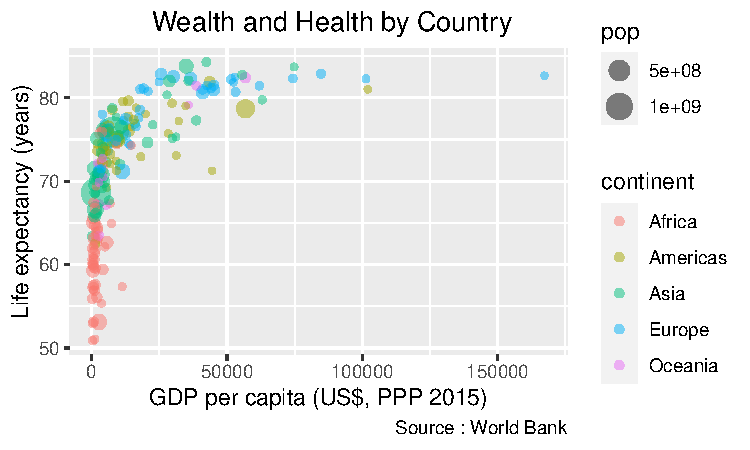
\includegraphics{Lec05_classnote_files/figure-latex/unnamed-chunk-3-1.pdf}

Poisson Distribution

\begin{Shaded}
\begin{Highlighting}[]
\NormalTok{y\_2 }\OtherTok{=} \FunctionTok{c}\NormalTok{()}
\ControlFlowTok{for}\NormalTok{ (i }\ControlFlowTok{in} \FunctionTok{c}\NormalTok{(}\DecValTok{1}\SpecialCharTok{:}\DecValTok{100000}\NormalTok{))\{}
\NormalTok{  x }\OtherTok{=} \FunctionTok{rpois}\NormalTok{(}\DecValTok{100}\NormalTok{,}\DecValTok{10}\NormalTok{)}
\NormalTok{  y\_2[i] }\OtherTok{=} \FunctionTok{mean}\NormalTok{(x)}
\NormalTok{\}}
\FunctionTok{hist}\NormalTok{(y\_2)}
\end{Highlighting}
\end{Shaded}

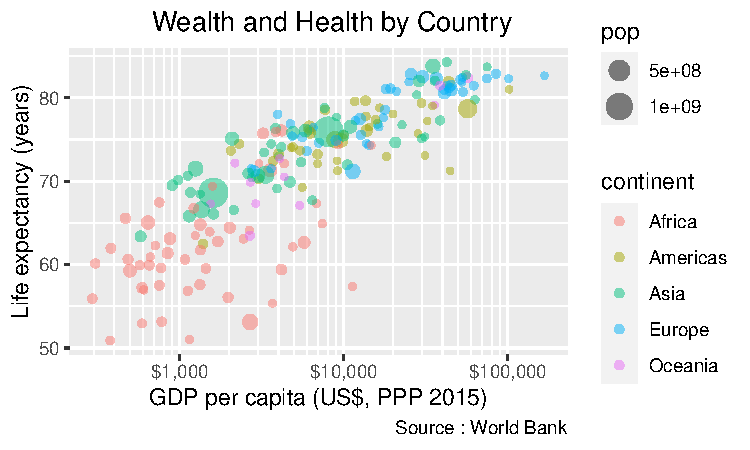
\includegraphics{Lec05_classnote_files/figure-latex/unnamed-chunk-4-1.pdf}

\hypertarget{binomial-distribution}{%
\subparagraph{Binomial Distribution}\label{binomial-distribution}}

\begin{Shaded}
\begin{Highlighting}[]
\NormalTok{y\_3 }\OtherTok{=} \FunctionTok{c}\NormalTok{()}
\ControlFlowTok{for}\NormalTok{ (i }\ControlFlowTok{in} \FunctionTok{c}\NormalTok{(}\DecValTok{1}\SpecialCharTok{:}\DecValTok{100000}\NormalTok{))\{}
\NormalTok{  x }\OtherTok{=} \FunctionTok{rbinom}\NormalTok{(}\DecValTok{100}\NormalTok{,}\DecValTok{10}\NormalTok{,}\FloatTok{0.5}\NormalTok{)}
\NormalTok{  y\_3[i] }\OtherTok{=} \FunctionTok{mean}\NormalTok{(x)}
\NormalTok{\}}
\FunctionTok{hist}\NormalTok{(y\_3)}
\end{Highlighting}
\end{Shaded}

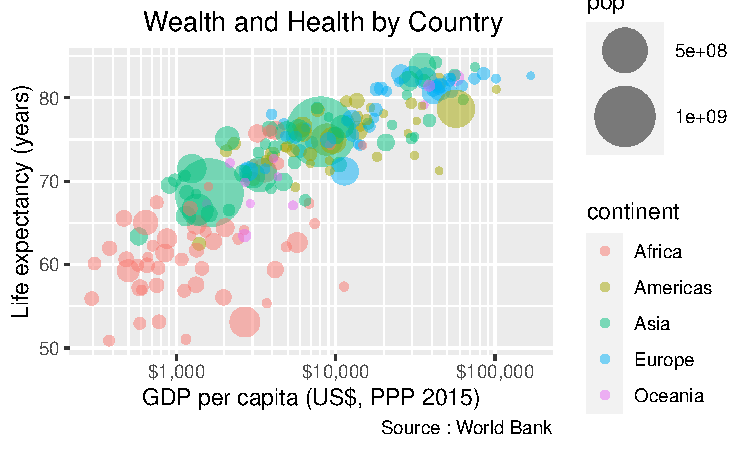
\includegraphics{Lec05_classnote_files/figure-latex/unnamed-chunk-5-1.pdf}

\hypertarget{genetics}{%
\subparagraph{Genetics}\label{genetics}}

Sum of the multiple independent variables leads to normal distribution
regression to the mean

\hypertarget{assumption}{%
\subparagraph{Assumption}\label{assumption}}

\begin{enumerate}
\def\labelenumi{\arabic{enumi}.}
\tightlist
\item
  assuming normality is critical for \textbf{parametric hypothesis test}
\item
  we use these test even when the distribution is non-normal - as long
  as the sample size is large enough
\end{enumerate}

Galton's box

The sum of the probability of a ball going left or right eventually
converges to a normal distribution.

\hypertarget{regression-to-the-mean}{%
\paragraph{Regression to the Mean}\label{regression-to-the-mean}}

If two very two people have kids, the kids tend to be taller than
average, but not as tall as the parents (same applies to intelligence).

The tall parents tend to have children that are closer to the mean of
the population.

in any series of random events an extraordinary event is more likely to
be followed, due to chance, by any more ordinary one.

the more extreme a variable is upon its first measurement, the more
likely it is to be closer to the average the second time it is measured.

\hypertarget{confidence-interval}{%
\paragraph{Confidence Interval}\label{confidence-interval}}

\begin{Shaded}
\begin{Highlighting}[]
\NormalTok{gen\_1 }\OtherTok{=} \FunctionTok{c}\NormalTok{()}

\ControlFlowTok{for}\NormalTok{ (i }\ControlFlowTok{in} \FunctionTok{c}\NormalTok{(}\DecValTok{1}\SpecialCharTok{:}\DecValTok{10}\NormalTok{))\{}
\NormalTok{  x }\OtherTok{=} \FunctionTok{mean}\NormalTok{(}\FunctionTok{rnorm}\NormalTok{(}\DecValTok{10}\NormalTok{,}\DecValTok{70}\NormalTok{,}\DecValTok{3}\NormalTok{))}
\NormalTok{  gen\_1[i] }\OtherTok{=}\NormalTok{ x}
\NormalTok{\}}
\FunctionTok{hist}\NormalTok{(gen\_1)}
\end{Highlighting}
\end{Shaded}

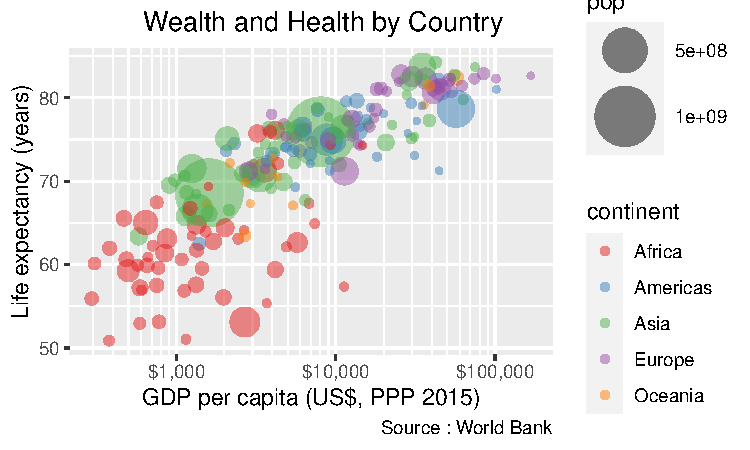
\includegraphics{Lec05_classnote_files/figure-latex/unnamed-chunk-6-1.pdf}

\begin{Shaded}
\begin{Highlighting}[]
\NormalTok{gen\_2 }\OtherTok{=} \FunctionTok{c}\NormalTok{()}

\ControlFlowTok{for}\NormalTok{ (i }\ControlFlowTok{in} \FunctionTok{c}\NormalTok{(}\DecValTok{1}\SpecialCharTok{:}\DecValTok{10}\NormalTok{))\{}
\NormalTok{  x }\OtherTok{=} \FunctionTok{mean}\NormalTok{(}\FunctionTok{rnorm}\NormalTok{(}\DecValTok{50}\NormalTok{,}\DecValTok{70}\NormalTok{,}\DecValTok{3}\NormalTok{))}
\NormalTok{  gen\_2[i] }\OtherTok{=}\NormalTok{ x}
\NormalTok{\}}
\FunctionTok{hist}\NormalTok{(gen\_2)}
\end{Highlighting}
\end{Shaded}

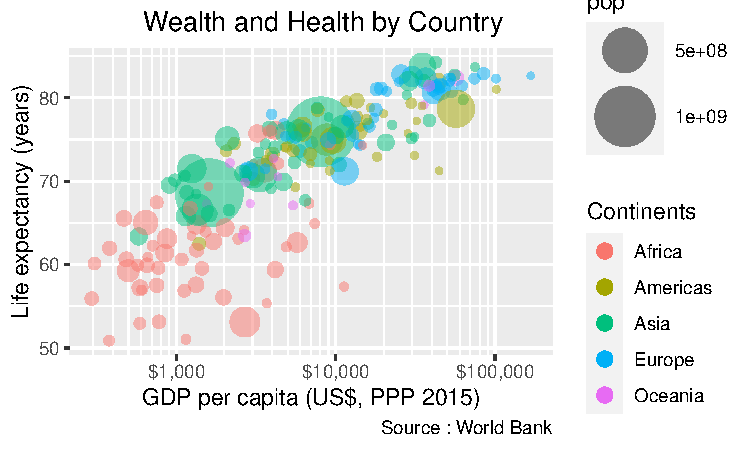
\includegraphics{Lec05_classnote_files/figure-latex/unnamed-chunk-7-1.pdf}

\begin{Shaded}
\begin{Highlighting}[]
\NormalTok{gen\_3 }\OtherTok{=} \FunctionTok{c}\NormalTok{()}

\ControlFlowTok{for}\NormalTok{ (i }\ControlFlowTok{in} \FunctionTok{c}\NormalTok{(}\DecValTok{1}\SpecialCharTok{:}\DecValTok{10}\NormalTok{))\{}
\NormalTok{  x }\OtherTok{=} \FunctionTok{mean}\NormalTok{(}\FunctionTok{rnorm}\NormalTok{(}\DecValTok{10}\NormalTok{,}\DecValTok{70}\NormalTok{,}\DecValTok{10}\NormalTok{))}
\NormalTok{  gen\_3[i] }\OtherTok{=}\NormalTok{ x}
\NormalTok{\}}
\FunctionTok{hist}\NormalTok{(gen\_3)}
\end{Highlighting}
\end{Shaded}

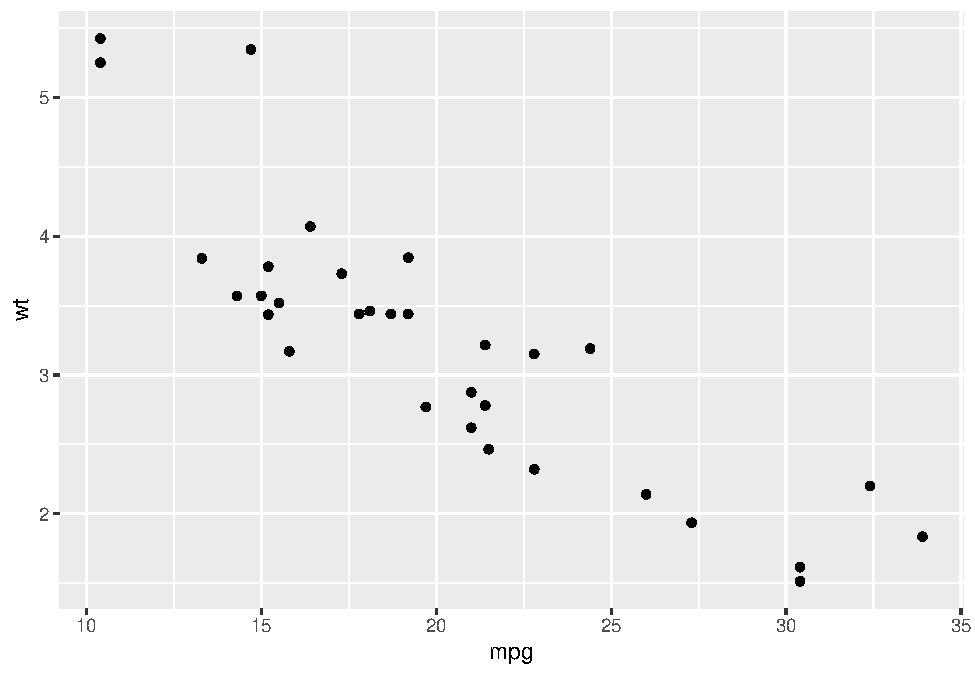
\includegraphics{Lec05_classnote_files/figure-latex/unnamed-chunk-8-1.pdf}

\begin{Shaded}
\begin{Highlighting}[]
\NormalTok{gen\_4 }\OtherTok{=} \FunctionTok{c}\NormalTok{()}

\ControlFlowTok{for}\NormalTok{ (i }\ControlFlowTok{in} \FunctionTok{c}\NormalTok{(}\DecValTok{1}\SpecialCharTok{:}\DecValTok{10}\NormalTok{))\{}
\NormalTok{  x }\OtherTok{=} \FunctionTok{mean}\NormalTok{(}\FunctionTok{rnorm}\NormalTok{(}\DecValTok{10}\NormalTok{,}\DecValTok{70}\NormalTok{,}\DecValTok{10}\NormalTok{))}
\NormalTok{  gen\_4[i] }\OtherTok{=}\NormalTok{ x}
\NormalTok{\}}
\FunctionTok{hist}\NormalTok{(gen\_4)}
\end{Highlighting}
\end{Shaded}

\includegraphics{Lec05_classnote_files/figure-latex/unnamed-chunk-9-1.pdf}

\end{document}
